\documentclass{ieeeojies}
\usepackage{etoolbox}
\usepackage{cite}
\usepackage{amsmath,amssymb,amsfonts}
\usepackage{algorithmic}
\usepackage{graphicx}
\usepackage{textcomp}
\usepackage{array}
\usepackage[table]{xcolor}
\usepackage{multirow}
\usepackage{multicol}
\usepackage{float}
\usepackage{hyperref}
\usepackage{breakurl}

\def\BibTeX{{\rm B\kern-.05em{\sc i\kern-.025em b}\kern-.08em
    T\kern-.1667em\lower.7ex\hbox{E}\kern-.125emX}}





\begin{document}
\title{Using Forecasting Models in Cryptocurrency Price Prediction}

\author{\uppercase{Hoang Nhat Minh}\authorrefmark{1},
\uppercase{Le Nguyen Nhat Minh\authorrefmark{2}, and Tran Thi Luyen}\authorrefmark{3}}

\address[1]{Faculty of Information Systems, University of Information Technology, (e-mail: 21522336@gm.uit.edu.vn)}
\address[2]{Faculty of Information Systems, University of Information Technology, (e-mail: 21522338@gm.uit.edu.vn)}
\address[3]{Faculty of Information Systems, University of Information Technology, (e-mail: 21521107@gm.uit.edu.vn)}

\markboth
{Author \headeretal: Hoang Nhat Minh, Le Nguyen Nhat Minh, Tran Thi Luyen}
{Author \headeretal: Hoang Nhat Minh, Le Nguyen Nhat Minh, Tran Thi Luyen}

\begin{abstract}
Predicting cryptocurrency price has become a central focus for investors and traders in the rapidly evolving landscape of digital assets. Cryptocurrencies like Bitcoin, Ethereum, and other altcoins have captured global attention, with their prices subject to fluctuations influenced by various factors, from market sentiment to technological developments. With the unprecedented volatility of these markets, the need for accurate forecasting models has never been more crucial. In this research, we conduct an in-depth analysis using various models including Linear regression (LR), Autoregressive Integrated Moving Average (ARIMA), Recurrent Neural Network (RNN), Gated Recurrent Unit (GRU), Long Short-Term Memory (LSTM), Seasonal Autoregressive Integrated Moving Average with eXogenous factors (SARIMAX), Neural Basis Expansion Analysis Time Series (NBEATS), Random Forest (RF) to predict prices of Bitcoin, Ethereum and BNB.
\end{abstract}

\begin{keywords}
Cryptocurrency price prediction, Bitcoin, Ethereum, BNB, Linear Regression, ARIMA, RNN, GRU, LSTM, SARIMAX, NBEATS, Random Forest.
\end{keywords}

\titlepgskip=-15pt

\maketitle

\section{Introduction}
\label{sec:introduction}
Cryptocurrency, a digital form of currency, has transformed the traditional concept of money. Unlike cash, cryptocurrencies exist purely in electronic form, utilizing encryption techniques for secure transactions. Bitcoin, the pioneering cryptocurrency introduced in 2009 by Satoshi Nakamoto, paved the way for a myriad of digital currencies that followed. The decentralized nature of cryptocurrencies means they operate without a central authority, using blockchain technology to record and verify transactions across a network of computers. This decentralization provides a level of transparency and security previously unseen in financial systems. As interest and adoption continue to grow, cryptocurrencies are reshaping the landscape of finance, offering individuals around the globe new avenues for transactions, investments, and financial freedom. \newline
By using forecasting models and machine learning algorithms to analyze historical data of Bitcoin, Ethereum, and BNB, the research objective is to provide valuable insights for investors and traders to forecast the cryptocurrency price movement. To evaluate the performance of each predictive model, we use three evaluation metrics Mean Absolute Error (MAE), Mean Absolute Percentage Error (MAPE), and Root Mean Squared Error (RMSE).
\section{Related Works}
Mahir Iqbal and his team \cite{b1} applied a machine learning based time series analysis in predicting the price of Bitcoin. They used ARIMA, FBProphet, and XG Boosting for time series analysis and evaluated these models by using three parameters RMSE, MAE, and R Squared (R\textsuperscript{2}). After conducting the analysis, they concluded that ARIMA is the best of three with RMSE score and MAE score are 322.4 and 227.3 respectively.\newline

Harsha Nanda Gudavalli and Khetan Venkata Ratnam Kancherla \cite{b2} identified four machine learning algorithms RF, Gradient Boosting (GB), LSTM, and GRU to make long-term predictions of cryptocurrency prices. Overall, LSTM is the most accurate model based on RMSE score of 0.01083, MSE score of 0.00011, and R Squared score of 0.80618.\newline

Junyi Zhu \cite{b3} applied LR for Bitcoin price prediction with the accuracy rate for training RSS and testing RSS are 94.6\% and 96.99\% respectively.\newline

Namrata Hemraj Gawali \cite{b4} developed predictive models to predict the price of Bitcoin using LSTM, Seasonal Autoregressive Integrated Moving Average (SARIMA), SARIMAX, and RNN. In conclusion, LSTM outperformed all other models with R Squared score of 0.9519, MAE score of 2476.68, MSE score of 10958440.29 and RMSE score of 3310.35.\newline

Alikhan Bulatov \cite{b5} used N-BEATS trained on Bitcoin daily, hourly, and up-to-the-minute data in comparison with LSTM and ARIMA. In this analysis, it is concluded that N-BEATS is the best model for forecasting the Bitcoin price with the RMSE score in daily, hourly, and minute data are 308.859, 59.303, and 13.678 respectively.\newline

\section{Materials}
\subsection{Dataset}
This research focuses on analyzing cryptocurrency trends through three data sets of three cryptocurrencies:
\begin{itemize}
	\item BTC/USD
	\item ETH/USD
	\item BNB/USD
\end{itemize}
Those data sets are extracted from the website \textit{investing.com} with the selected period from March 1, 2019, to June 1, 2024. 
Each data set contains 1920 data rows and has 6 attributes:
\begin{itemize}
	\item Price: The last transacted price in a day.
	\item Open: The opening price in a day.
	\item High: The highest price in a day.
	\item Low: The lowest price in a day.
	\item Vol: The total amount traded in a day.
	\item Change \%: The percentage change in the closing price compared to the previous day’s closing price.
\end{itemize}
\subsection{Descriptive Statistics}
\begin{table}[H]
	\centering
	\caption{BTC, ETH, BNB’s Descriptive Statistics}
	\begin{tabular}{|>{\columncolor{red!20}}c|c|c|c|}
		\hline
		\rowcolor{red!20} & BTC & ETH & BNB \\ \hline
		Count & 1920 & 1920 & 1920 \\ \hline
		Mean & 27916.88 & 1580.30 & 229.54\\ \hline
		Std & 17918.78 & 1205.85 & 184.43\\ \hline
		Min & 3715 & 107.58 & 9.28\\ \hline
		25\% & 10434.10 & 268.88 & 27.03\\ \hline
		50\% & 25933.90 & 1622.45 & 247.55\\ \hline
		75\% & 41492.60 & 2333.36 & 332.12\\ \hline
		Max & 73060.80 & 4808.09 & 676.12\\ \hline
	\end{tabular}
\end{table}

\begin{figure}[H]
	\centering
	\begin{minipage}{0.23\textwidth}
		\centering
		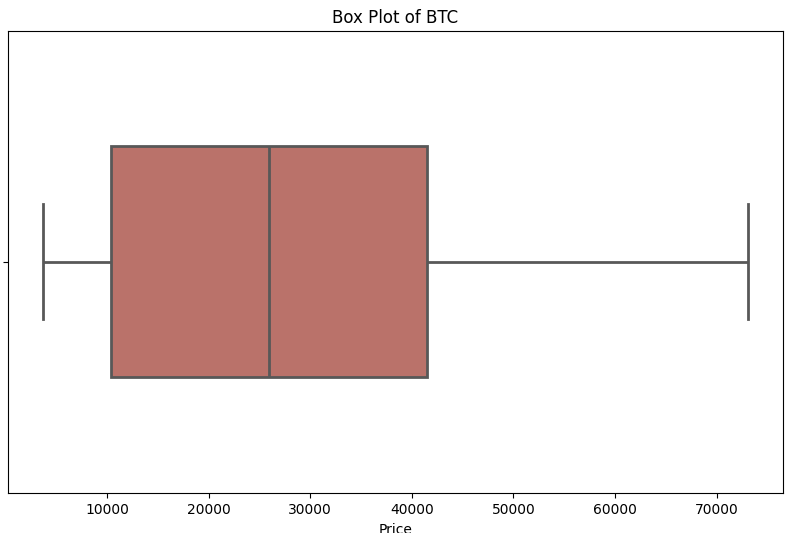
\includegraphics[width=1\textwidth]{bibliography/Images/BoxPlot_BTC.PNG}
		\caption{Bitcoin price's boxplot}
		\label{fig:1}
	\end{minipage}
	\hfill
	\begin{minipage}{0.23\textwidth}
		\centering
		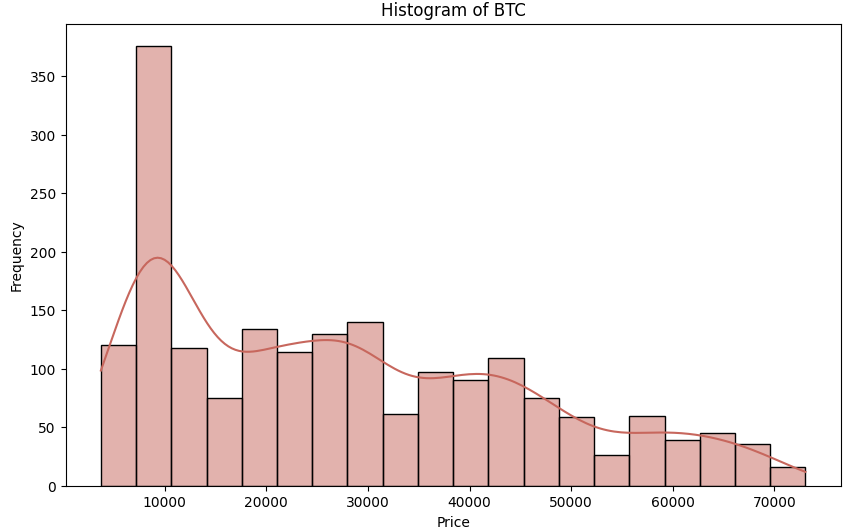
\includegraphics[width=1\textwidth]{bibliography/Images/Histogram_BTC.PNG}
		\caption{Bitcoin price's histogram}
		\label{fig:2}
	\end{minipage}
\end{figure}

\begin{figure}[H]
	\centering
	\begin{minipage}{0.23\textwidth}
		\centering
		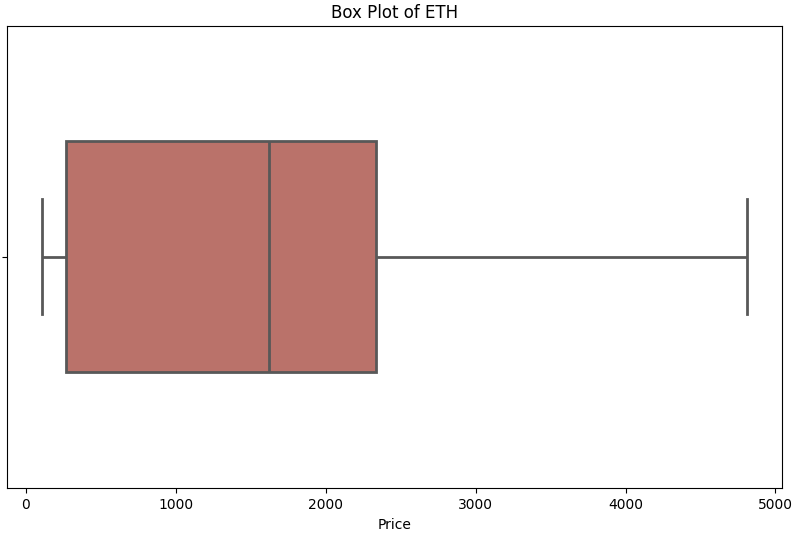
\includegraphics[width=1\textwidth]{bibliography/Images/BoxPlot_ETH.PNG}
		\caption{Ethereum price's boxplot}
		\label{fig:1}
	\end{minipage}
	\hfill
	\begin{minipage}{0.23\textwidth}
		\centering
		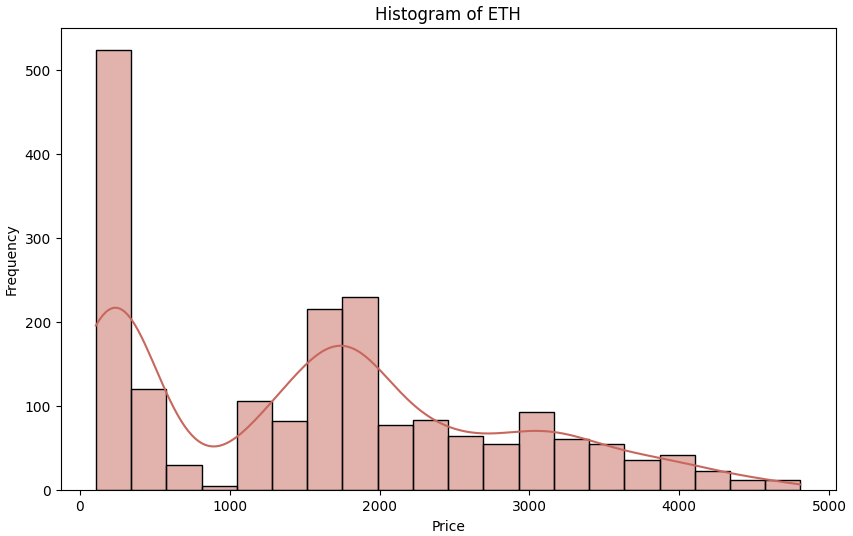
\includegraphics[width=1\textwidth]{bibliography/Images/Histogram_ETH.PNG}
		\caption{Ethereum price's histogram}
		\label{fig:2}
	\end{minipage}
\end{figure}

\begin{figure}[H]
	\centering
	\begin{minipage}{0.23\textwidth}
		\centering
		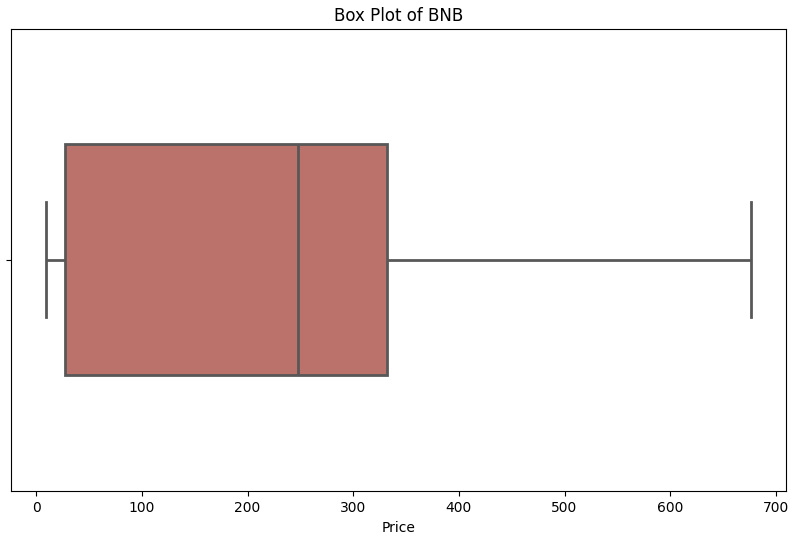
\includegraphics[width=1\textwidth]{bibliography/Images/BoxPlot_BNB.PNG}
		\caption{BNB price's boxplot}
		\label{fig:1}
	\end{minipage}
	\hfill
	\begin{minipage}{0.23\textwidth}
		\centering
		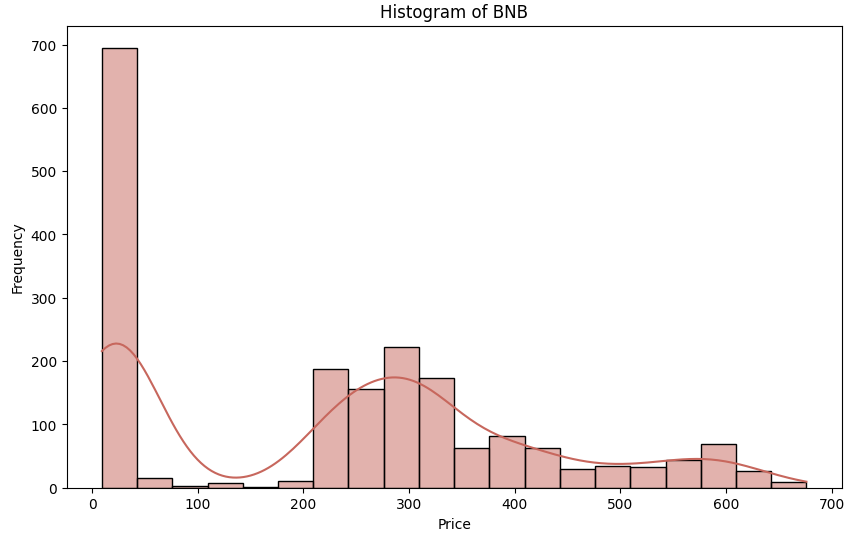
\includegraphics[width=1\textwidth]{bibliography/Images/Histogram_BNB.PNG}
		\caption{BNB price's histogram}
		\label{fig:2}
	\end{minipage}
\end{figure}
\section{Methodology}
\subsection{Linear regression}
Linear regression \cite{b6} is an algorithm that provides a linear relationship between an independent variable and a dependent variable. A linear regression model with more than one independent variable is called a multiple linear regression model. A multiple linear regression model has the form:
\newline  \centerline{$\textit{Y} = \beta_{0} + \beta_{1}X_{1} + \beta_{2}X_{2} + ... + \beta_{k}X_{k} + \varepsilon$}
\newline Where:
\begin{itemize}
	\item \textit{Y} is the dependent variable.
	\item $X_{1},...,X_{k}$ are the independent (explanatory) variables.
	\item $\beta_{0}$ is the intercept term.
	\item $\beta_{1},...,\beta_{k}$ are the regression coefficients for the independent variables.
	\item $\varepsilon$ is the error term.
\end{itemize}

\subsection{Autoregressive Integrated Moving Average (ARIMA)}
ARIMA \cite{b7}, which stands for AutoRegressive Integrated Moving Average, is a statistical analysis model designed to analyze time series data. It helps in understanding the data set more comprehensively and predicting future trends. The complete model is represented as follows:
\newline \centerline{$y'_{t} = c + \phi_{1}y'_{t-1} + ... + \phi_{p}y'_{t-p} + \theta_{1}\varepsilon_{t-1} + ... + \theta_{q}\varepsilon_{t-q} + \varepsilon_{t}$}
\newline Where:
\begin{itemize}
	\item $y'_{t}$ is the value of the time series at time \textit{t}.
	\item \textit{c} is the constant term.
	\item $\phi_{1},...,\phi_{p}$ are the autoregressive coefficients.
	\item $\theta_{1},...,\theta_{q}$ are the moving average coefficients.
	\item $\varepsilon_{t}$ is the white noise at time \textit{t}.
\end{itemize}
A non - seasonal ARIMA model is classified as an ARIMA (p, d, q) model, where:
\begin{itemize}
	\item \textit{p} is the number of lag observations included in the model.
	\item \textit{d} is the number of times that the raw observations are differenced.
	\item \textit{q} is the size of the moving average window, also called the order of moving average.
\end{itemize}
\subsection{Autoregressive Integrated Moving Average with eXogenous factors (SARIMAX)}
SARIMAX \cite{b8}, which stands for Seasonal Autoregressive Integrated Moving Average with eXogenous factors, is an enhanced version of the SARIMA model, incorporating external feature parameters (X) to improve performance. By including exogenous factors, SARIMAX reduces prediction errors, addresses autocorrelation issues, and enhances prediction accuracy. The model captures both seasonal effects and exogenous factors, represented as SARIMAX (p, d, q) * (P, D, Q), with the exogenous factors being optional parameters. These factors provide additional details to support and refine the prediction model. The SARIMAX can be represented as follows:
\newline \centerline{$d_{t} = c + \displaystyle \sum_{n=1}^{p}\alpha_{n}d_{t-n} + \displaystyle \sum_{n=1}^{q}\theta_{n}\epsilon_{t-n} + \displaystyle \sum_{n=1}^{r}\beta_{n}x_{n_{t}}$}
\newline \centerline{$+ \displaystyle \sum_{n=1}^{P}\phi_{n}d_{t-sn} + \displaystyle \sum_{n=1}^{Q}\eta_{n}\epsilon_{t-sn} + \epsilon_{t}$}
\newline Where:
\begin{itemize}
	\item \textit{P} is seasonal autoregressive order.
	\item \textit{D} is seasonal differencing order.
	\item \textit{Q} is seasonal moving average order.
	\item \textit{s} is the length of the seasonal cycle.
\end{itemize}
\subsection{Random Forest}
Random Forest \cite{b9} is an ensemble learning method used for classification, regression, and various other tasks. It works by constructing numerous decision trees during training and then outputs either the mode of the classes for classification tasks or the mean prediction for regression tasks, based on the individual trees' results.
\begin{figure}[H]
	\centering
	\begin{minipage}{0.23\textwidth}
		\centering
		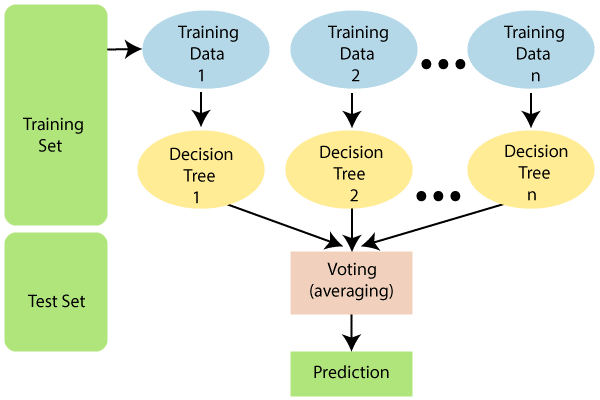
\includegraphics[width=1\textwidth]{bibliography/Images/RandomForest_Img1.png}
		\caption{The structure of Random Forest model}
		\label{fig:1}
	\end{minipage}
\end{figure}
Each tree in a random forest samples subsets of the training data randomly through a process called bootstrap aggregating. The model is then fitted to these smaller data sets, and the predictions are aggregated. This method allows multiple instances of the same data to be used repeatedly through replacement sampling. As a result, the trees are trained on different sets of data and utilize different features for decision-making.
\begin{figure}[H]
	\centering
	\begin{minipage}{0.23\textwidth}
		\centering
		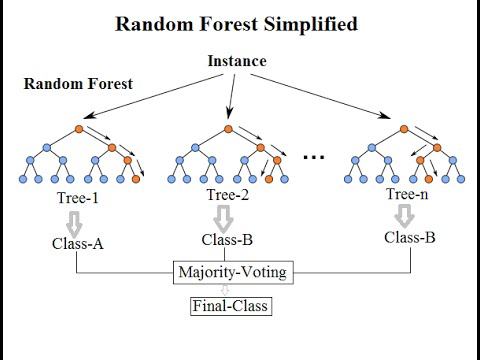
\includegraphics[width=1\textwidth]{bibliography/Images/RandomForest_Img2.png}
		\caption{Overview of Random Forest model}
		\label{fig:1}
	\end{minipage}
\end{figure}
The following steps explain the working Random Forest algorithm:
\begin{enumerate}
	\item From the original dataset, select random samples of data .
	\item Train a decision tree model on each sample.
	\item For each tree, select a random subset of features to consider at each split.
	\item Combine the individual decision trees into a final model by taking a majority vote for classification or averaging for regression.
\end{enumerate}
\subsection{Recurrent Neural Network (RNN)}
Recurrent Neural Networks \cite{b10} (RNNs) are a type of artificial neural network specifically designed for processing sequential data. Unlike traditional feedforward neural networks, RNNs have cyclic connections that enable them to retain a memory of previous inputs.
\begin{figure}[H]
	\centering
	\begin{minipage}{0.32\textwidth}
		\centering
		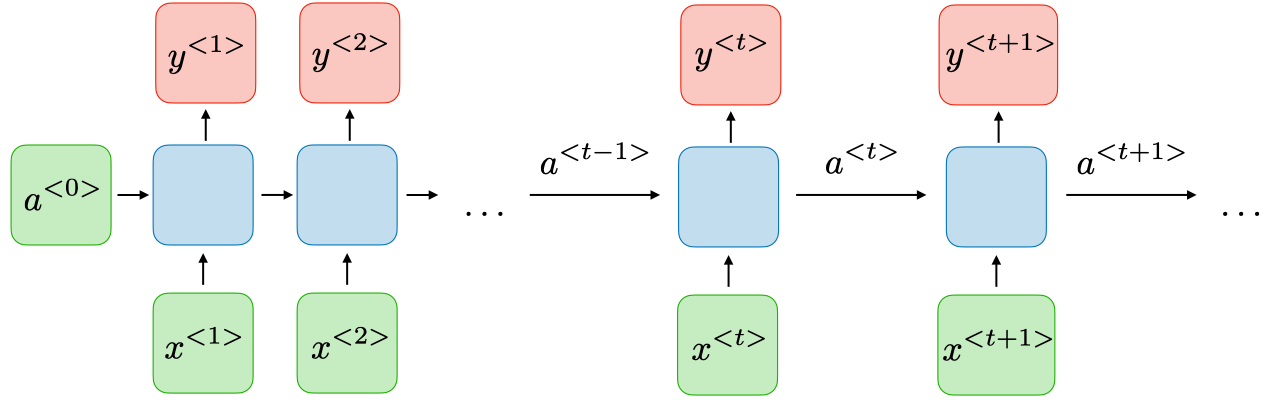
\includegraphics[width=1\textwidth]{bibliography/Images/RNN_Img1.png}
		\caption{Overview of Recurrent Neural Network}
		\label{fig:1}
	\end{minipage}
\end{figure}
For each timestep \textit{t}, the activation $a^{<t>}$ and the output $y^{<t>}$ are expressed as follows:
\newline \centerline{$a^{<t>} = g_{1}(W_{aa}a^{<t-1>} + W_{ax}x^{<t>} + b_{a})$}
\newline and
\newline \centerline{$y^{<t>} = g_{2}(W_{ya}a^{<t>} +b_{y})$}
\newline Where:
\begin{itemize}
	\item $W_{ax}, W_{as}, W_{ya}, b_{a}, b_{y}$ are coefficients that are shared temporally.
	\item $g_{1}, g_{2}$ are activation functions.
\end{itemize}
\begin{figure}[H]
	\centering
	\begin{minipage}{0.32\textwidth}
		\centering
		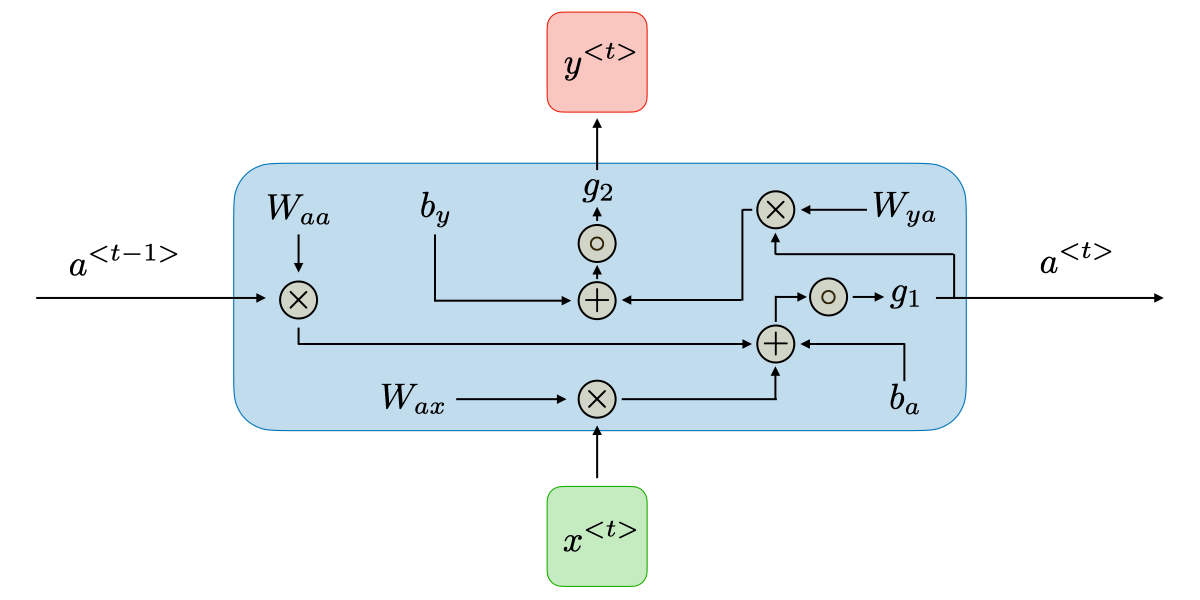
\includegraphics[width=1\textwidth]{bibliography/Images/RNN_Img2.png}
		\caption{Architecture of a traditional RNN}
		\label{fig:1}
	\end{minipage}
\end{figure}
For a recurrent neural network, the loss function $\mathcal{L}$ over all time steps is defined based on the loss at each individual time step:
\newline \centerline{$\mathcal{L}(\hat{y},y) = \displaystyle \sum_{t=1}^{T_{y}}\mathcal{L}(\hat{y}^{<t>},y^{<t>})$}
Backpropagation is done at each point in time. At timestep \textit{T}, the derivative of the loss $\mathcal{L}$ with respect to weight matrix \textit{W} is expressed as follows:
\newline \centerline{$\displaystyle \frac{\partial \mathcal{L}^{(T)}}{\partial W} = \displaystyle \sum_{t=1}^{T} \left. \frac{\partial \mathcal{L}^{(T)}}{\partial W} \right|_{(t)}$}
\subsection{Long Short-Term Memory (LSTM)}
Long Short-Term Memory \cite{b11} (LSTM) networks are a type of Recurrent Neural Network (RNN) designed to capture long-term dependencies in sequential data. LSTMs can process and analyze various forms of sequential data, including time series, text, and speech. They utilize a memory cell and gates to regulate the flow of information, enabling them to selectively retain or discard information as necessary. This mechanism helps them avoid the vanishing gradient problem that affects traditional RNNs.
\begin{figure}[H]
	\centering
	\begin{minipage}{0.32\textwidth}
		\centering
		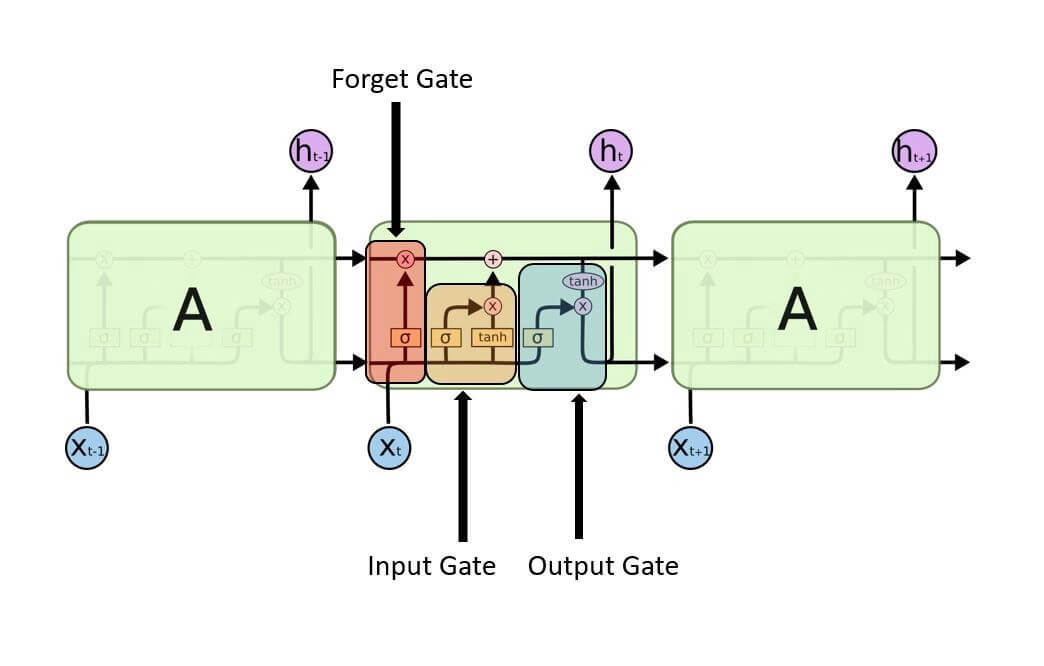
\includegraphics[width=1\textwidth]{bibliography/Images/LSTM_Img1.jpg}
		\caption{Architecture of LSTM}
		\label{fig:1}
	\end{minipage}
\end{figure}
LSTM have 4 different components: cell state (memory cell), forget gate, input gate, output gate.
\begin{figure}[H]
	\centering
	\begin{minipage}{0.32\textwidth}
		\centering
		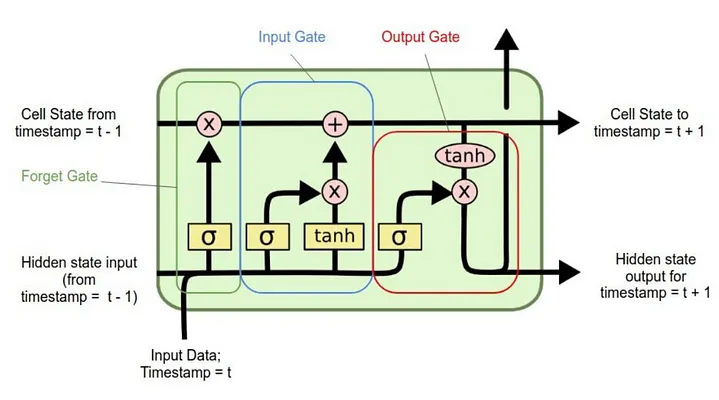
\includegraphics[width=1\textwidth]{bibliography/Images/LSTM_Img2.png}
		\caption{LSTM components}
		\label{fig:1}
	\end{minipage}
\end{figure}
\begin{itemize}
	\item  Forget gate: 
	\newline \centerline{$\textit{f}_{t} = \sigma (\textit{W}_{\textit{f}}.[h_{t-1},x_{t}] + b_{\textit{f}})$}
	\item Input gate: 
	\newline \centerline{$i_{t} = \sigma(\textit{W}_{i}.[h_{t-1},x_{t}]+b_{i})$}
	\newline \centerline{$\Tilde{C}_{t} = tanh(W_{C}.[h_{t-1},x_{t}] + b_{C})$}
	\item Output gate:
	\newline \centerline{$o_{t} = \sigma(W_{o}.[h_{t-1},x_{t}] + b_{o})$}
	\newline \centerline{$h_{t} = o_{t} * tanh(C_{t})$}
\end{itemize}
\subsection{Gated Recurrent Unit (GRU)}
A Gated Recurrent Unit \cite{b12} (GRU) is a type of recurrent neural network (RNN) architecture designed to model sequential data by selectively retaining or forgetting information over time. GRUs simplify the RNN structure by utilizing two main gates: the reset gate and the update gate. The reset gate controls how much of the previous hidden state should be forgotten, while the update gate decides how much of the candidate activation vector should be integrated into the new hidden state.
\begin{figure}[H]
	\centering
	\begin{minipage}{0.25\textwidth}
		\centering
		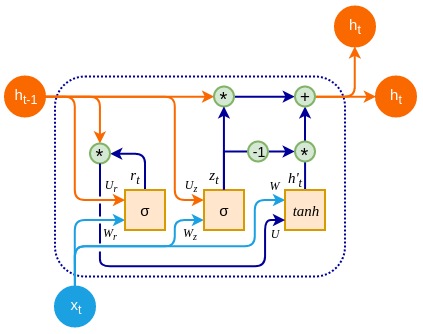
\includegraphics[width=1\textwidth]{bibliography/Images/GRU_Img1.png}
		\caption{Architecture of GRU}
		\label{fig:1}
	\end{minipage}
\end{figure}
A GRU cell has 4 components:
\begin{itemize}
	\item Reset gate:
	\newline \centerline{$r_{t} = \sigma(W_{r}x_{t} + U_{r}h_{t-1})$}
	\newline Where:
	\begin{itemize}
		\item $x_{t}$ is the current information.
		\item $h_{t-1}$ is the previous information.
		\item $W_{r}$ represents how much current information is weighted.
		\item $U_{r}$ represents how much previous information is weighted.
	\end{itemize}
	\item Update gate:
	\newline \centerline{$z_{t} = \sigma(W_{z}x_{t} + U_{z}h_{t-1})$}
	\newline Where:
	\begin{itemize}
		\item $x_{t}$ is the current information.
		\item $h_{t-1}$ is the previous information.
		\item $W_{z}$ represents how much current information is weighted.
		\item $U_{z}$ represents how much previous information is weighted.
	\end{itemize}
	\item New memory content:
	\newline \centerline{$h'_{t} =  tanh(W_{h}x_{t} + r_{t}.U_{h}h_{t-1})$}
	\newline Where:
	\begin{itemize}
		\item $x_{t}$ is the current information.
		\item $h_{t-1}$ is the previous information.
		\item $r_{t}$ represents how much previous information should be forgotten.
		\item $W_{h}$ represents how much current information is weighted.
		\item $U_{h}$ represents how much previous information is weighted.
	\end{itemize}
	\item Final memory content:
	\newline \centerline{$h_{t} =  z_{t}.h'_{t} + (1 - z_{t}).h_{t-1}$}
	\newline Where:
	\begin{itemize}
		\item $z_{t}$ represents how much the unit updates its information with the current information.
		\item $h_{t-1}$ represents the previous information.
		\item $h'_{t}$ represents the current information with some degree of dependency on the previous information.
	\end{itemize}
\end{itemize}


\subsection{Neural Basis Expansion Analysis Time Series (NBEATS)}
Neural Basis Expansion Analysis for Time Series \cite{b13} (NBEATS) is a deep learning architecture designed specifically for forecasting time series data. It uses deep neural networks to directly learn complex temporal patterns from the data.
\begin{figure}[H]
	\centering
	\begin{minipage}{0.25\textwidth}
		\centering
		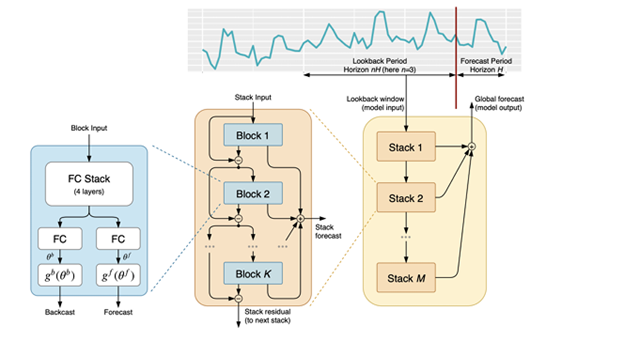
\includegraphics[width=1\textwidth]{bibliography/Images/NBEATS_Img1.png}
		\caption{Architecture of NBEATS}
		\label{fig:1}
	\end{minipage}
\end{figure}
\subsubsection{Basic building blocks}
Basic building blocks has a fork architecture with 1 input and 2 outputs. The input of the first block is overall model input n*H with H is the length used to predict future, and n is in the range [2,7]. With other blocks, the inputs of the model are residual outputs of the previous block. The basic building block is a multi-layer FC (Fully Connected) network with RELU (Rectified Linear Unit) nonlinearities. It predicts basis expansion coefficients both forward, $\theta^{f}$, (forecast) and backward, $\theta^{b}$,(backcast). The outputs of the block are backcast and forecast by  mapping 2 vector $\theta^{f}$ and $\theta^{b}$ using $g^{f}$ and $g^{b}$.
\subsubsection{Stacking blocks}
Basic building blocks are arranged into a single stack. The first basic block has two outputs: the backcast and forecast vectors. To calculate the input for the next block, the new look-back input is used in an element-wise subtraction of backcast. This subtraction yields a vector which incorporates only things not learned by the first block, which will be used as the input for the subsequent block.
\section{Result}
\subsection{Evaluation methods}
\textbf{Mean Absolute Percentage  Error} (MAPE) represents the average of the absolute percentage errors of each entry in a dataset to calculate how accurate the forecasted quantities were in comparison with the actual quantities.\\
\[ M = \frac{1}{n} \sum_{t=1}^{n} \left| \frac{A_{t} - F_{t}}{A_{t}} \right| \]
\newline Where:
\begin{itemize}
	\item \textit{n} is the number of forecast values.
	\item $A_{t}$ is the actual value of the time series at time \textit{t}.
	\item $F_{t}$ is the forecast value at time \textit{t}.
\end{itemize}
\textbf{Root Mean Squared Error} (RMSE) measures the average difference between a statistical model’s predicted values and the actual values. It quantifies how dispersed these residuals are, revealing how tightly the observed data clusters around the predicted values.\\
\[RMSE=\sqrt{\sum_{i=1}^{n} \frac{(\hat{y_i}-y_i )^2}{n} }\]\\
\newline Where:
\begin{itemize}
	\item $\hat{y_1}, \hat{y_2}, ..., \hat{y_n}$ are predicted values.
	\item ${y_1}, {y_2}, ..., {y_n}$ are observed values.
	\item \textit{n} is the number of observations.
\end{itemize}
\textbf{Mean Absolute Error} (MAE) measures the average of the magnitudes of the errors between the predicted and actual values.\\
\[MAE=\frac{1}{n}\sum_{i=1}^{n}|y_i - 
\hat{y_i}|\]
\newline Where:
\begin{itemize}
	\item \textit{n} is the number of observations.
	\item $y_i$ is the actual value of the $i^{th}$ observation.
	\item $\hat{y_i}$ is the predicted value of the $i^{th}$ observation.
\end{itemize}
\subsection{BTC/USD Dataset}
\begin{table}[H]
	\centering
	\begin{tabular}{|c|c|c|c|c|}
		\hline
		\multicolumn{5}{|c|}{\textbf{BTC/USD Dataset's Evaluation}}\\
		\hline
		\centering Model & Training:Testing & RMSE & MAPE (\%) & MAE\\
		\hline
		\multirow{2}{*}{LR} & 7:3 & 21064.65 &  74.50 &  19521.81 \\ & \textbf{8:2} & \textbf{13640.22} &  \textbf{29.98} &  \textbf{11686.03} \\ & 9:1 & 19141.51 & 25.41 & 15704.47\\
		\hline
		\multirow{2}{*}{ARIMA} & 7:3 & 22094.05 & 36.85 & 16069.35 \\ & \textbf{8:2} & \textbf{21759.27}& \textbf{28.62} & \textbf{15439.40} \\ & 9:1 & 21255.13 & 28.96 & 17740.84\\
		\hline
		\multirow{2}{*}{RNN} & 7:3& 1498.40 &  3.38 & 1205.54\\ & \textbf{8:2}& \textbf{1468.04} & \textbf{1.89} & \textbf{953.16} \\ & 9:1 & 2215.84 & 2.49& 1656.83\\
		\hline
		\multirow{2}{*}{GRU} & \textbf{7:3}	&  \textbf{1172.71} & \textbf{1.89} & \textbf{761.59} \\ & 8:2 & 1690.30 & 2.36 &  1186.07 \\ & 9:1 & 2164.76  & 2.48 & 1645.22\\
		\hline
		\multirow{2}{*}{LSTM} & 7:3 &  2375.04 &  4.42 & 1838.50 \\ & \textbf{8:2} &  \textbf{1652.29} & \textbf{2.13} &  \textbf{1098.40} \\ & 9:1 & 2846.96  & 3.48 & 2327.89\\
		\hline
		\multirow{2}{*}{SARIMAX} & 7:3	& 18939.08 & 29.80 & 13272.13 \\ & \textbf{8:2} & \textbf{18183.71} & \textbf{23.68} & \textbf{12728.52} \\ & 9:1 & 19199.60 & 25.88 & 15909.43\\
		\hline
		\multirow{2}{*}{NBEATS} & \textbf{7:3} & \textbf{1359.61} & \textbf{2.61} & \textbf{954.51} \\ & 8:2 & 1417.10 & 2.26 & 989.33 \\ & 9:1 & 1800.29	& 2.37 & 1337.98 \\
		\hline
		\multirow{2}{*}{RF} & \textbf{7:3} & \textbf{1890.12} & \textbf{3.18} & \textbf{1211.36} \\ & 8:2 & 2271.28 & 2.77 & 1390.68 \\ & 9:1 & 3063.31 & 3.51 & 2180.00 \\
		\hline
	\end{tabular}
	\caption{BTC/USD Dataset's Evaluation}
	\label{btcresult}
\end{table}
\begin{figure}[H]
	\centering
	\begin{minipage}{0.6\linewidth}
		\centering
		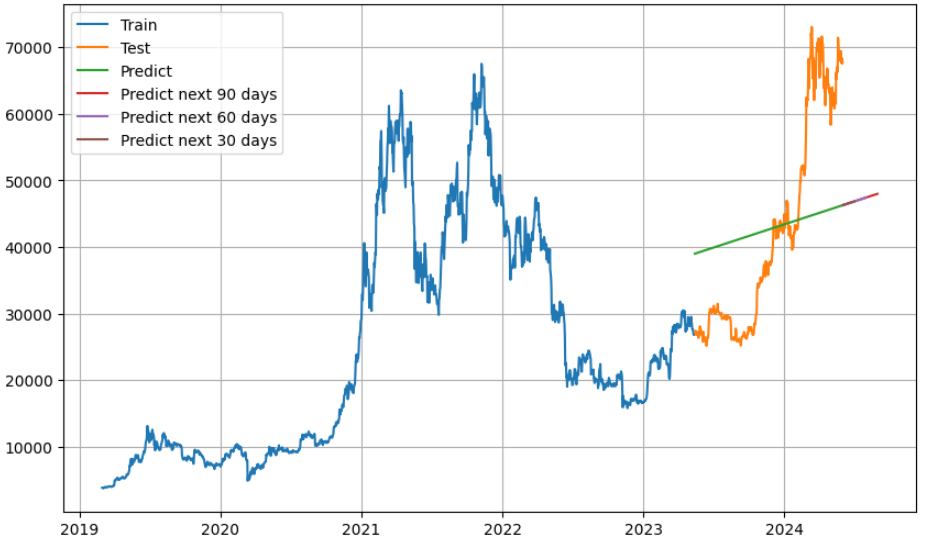
\includegraphics[width=\linewidth]{bibliography/Images/LR_BTC_82.PNG}
		\caption{LR model's result with 8:2 splitting proportion}
	\end{minipage}
\end{figure}
\begin{figure}[H]
	\centering
	\begin{minipage}{0.6\linewidth}
		\centering
		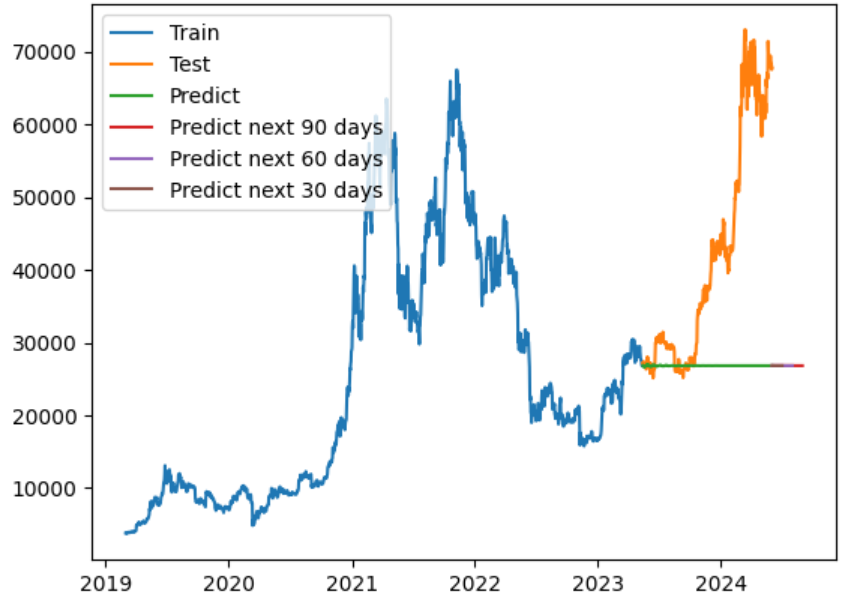
\includegraphics[width=\linewidth]{bibliography/Images/ARIMA_BTC_82.PNG}
		\caption{ARIMA model's result with 8:2 splitting proportion}
	\end{minipage}
\end{figure}
\begin{figure}[H]
	\centering
	\begin{minipage}{0.6\linewidth}
		\centering
		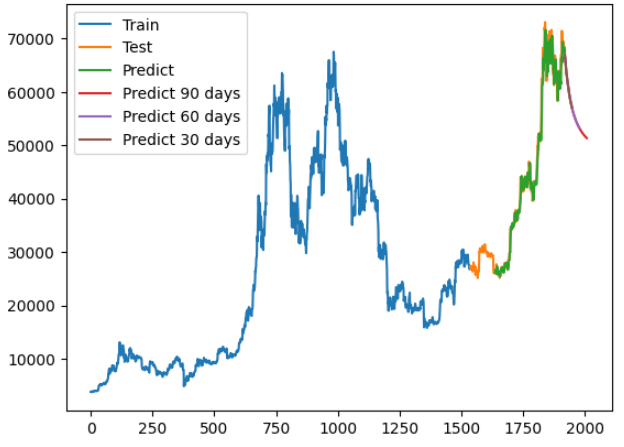
\includegraphics[width=\linewidth]{bibliography/Images/RNN_BTC_82.PNG}
		\caption{RNN model's result with 8:2 splitting proportion}
	\end{minipage}
\end{figure}
\begin{figure}[H]
	\centering
	\begin{minipage}{0.6\linewidth}
		\centering
		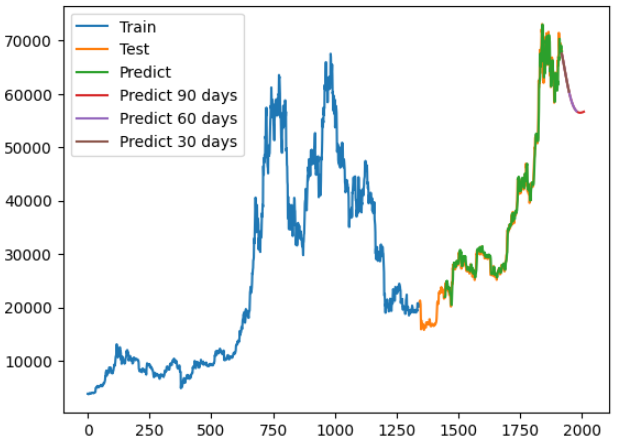
\includegraphics[width=\linewidth]{bibliography/Images/GRU_BTC_73.PNG}
		\caption{GRU model's result with 7:3 splitting proportion}
	\end{minipage}
\end{figure}
\begin{figure}[H]
	\centering
	\begin{minipage}{0.6\linewidth}
		\centering
		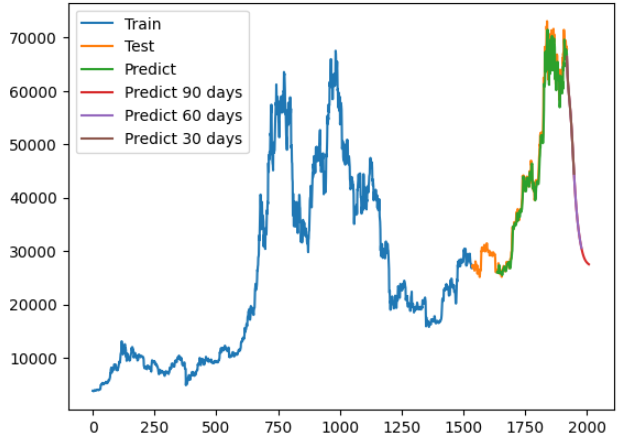
\includegraphics[width=\linewidth]{bibliography/Images/LSTM_BTC_82.PNG}
		\caption{LSTM model's result with 8:2 splitting proportion}
	\end{minipage}
\end{figure}
\begin{figure}[H]
	\centering
	\begin{minipage}{0.6\linewidth}
		\centering
		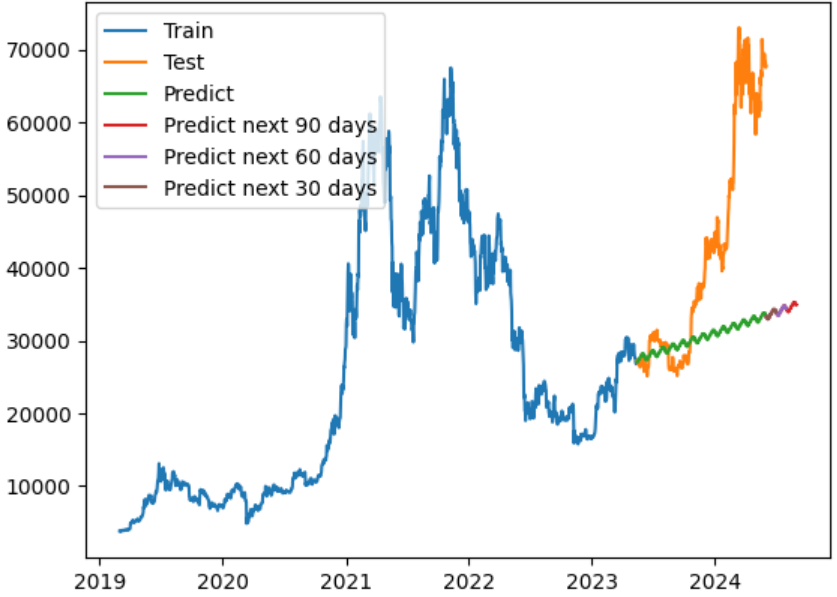
\includegraphics[width=\linewidth]{bibliography/Images/SARIMAX_BTC_82.PNG}
		\caption{SARIMAX model's result with 8:2 splitting proportion}
	\end{minipage}
\end{figure}
\begin{figure}[H]
	\centering
	\begin{minipage}{0.6\linewidth}
		\centering
		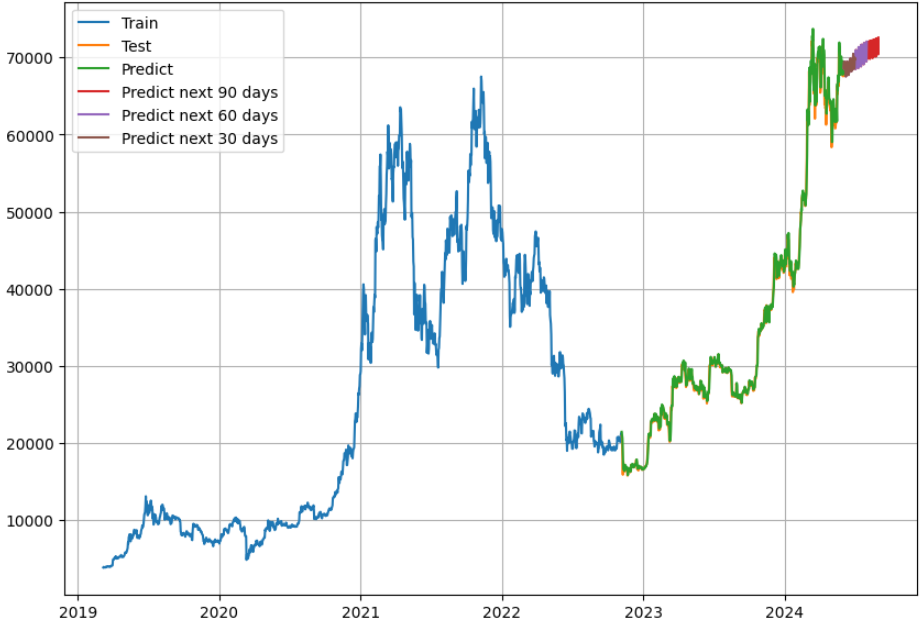
\includegraphics[width=\linewidth]{bibliography/Images/NBEATS_BTC_73.PNG}
		\caption{NBEATS model's result with 7:3 splitting proportion}
	\end{minipage}
\end{figure}
\begin{figure}[H]
	\centering
	\begin{minipage}{0.6\linewidth}
		\centering
		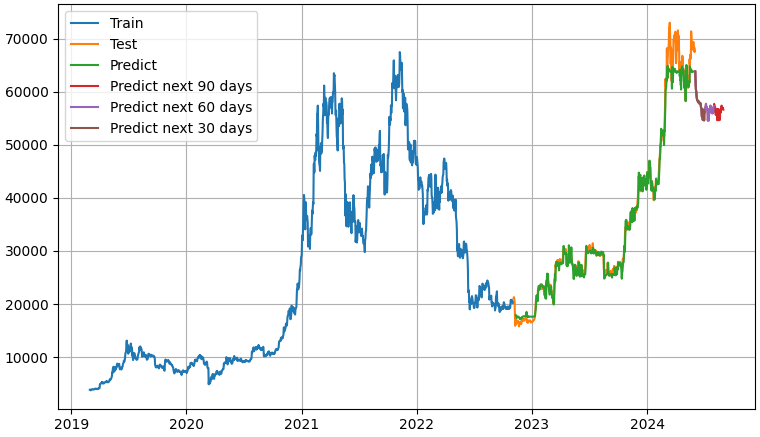
\includegraphics[width=\linewidth]{bibliography/Images/RF_BTC_73.PNG}
		\caption{RF model's result with 7:3 splitting proportion}
	\end{minipage}
\end{figure}

\subsection{ETH/USD Dataset}
\begin{table}[H]
	\centering
	\begin{tabular}{|c|c|c|c|c|}
		\hline
		\multicolumn{5}{|c|}{\textbf{ETH/USD Dataset's Evaluation}}\\
		\hline
		\centering Model & Training:Testing & RMSE & MAPE (\%) & MAE\\
		\hline
		\multirow{2}{*}{LR} & 7:3 & 1685.08 &  90.81 &  1634.17 \\ & 8:2 & 893.57 & 41.50 & 808.89 \\ & \textbf{9:1} & \textbf{547.36} & \textbf{15.64} & \textbf{466.42}\\
		\hline
		\multirow{2}{*}{ARIMA} & 7:3 & 887.16 & 24.79 & 618.80 \\ & \textbf{8:2} & \textbf{884.49}& \textbf{20.99} & \textbf{607.30} \\ & 9:1 & 1020.51 & 26.16 & 841.51\\
		\hline
		\multirow{2}{*}{RNN} & \textbf{7:3} & \textbf{76.95} & \textbf{2.32} & \textbf{52.98}\\ & 8:2& 89.69 & 2.17 & 58.29 \\ & 9:1 & 132.16 & 2.73 & 92.83\\
		\hline
		\multirow{2}{*}{GRU} & \textbf{7:3}	& \textbf{74.03} &  \textbf{1.95} &  \textbf{46.39} \\ & 8:2 & 89.12 & 2.43 & 62.01 \\ & 9:1 & 145.64  & 3.15 & 107.97\\
		\hline
		\multirow{2}{*}{LSTM} & 7:3 &  92.94 &  2.64 & 63.26 \\ & \textbf{8:2} &  \textbf{88.47} & \textbf{2.15} &  \textbf{57.68} \\ & 9:1 & 131.42  & 2.75 & 93.08\\
		\hline
		\multirow{2}{*}{SARIMAX} & \textbf{7:3}	& \textbf{642.09} & \textbf{16.96} &  \textbf{421.99} \\ & 8:2 & 670.58 & 16.65 & 460.51 \\ & 9:1 & 938.35 &  24.06 & 773.16\\
		\hline
		\multirow{2}{*}{NBEATS} & 7:3 & 79.98 & 2.53 & 54.32 \\ & \textbf{8:2} & \textbf{78.58} & \textbf{1.99} & \textbf{49.91} \\ & 9:1 & 126.87	& 3.19 & 94.92 \\
		\hline
		\multirow{2}{*}{RF} & \textbf{7:3} & \textbf{77.44} & \textbf{2.43} & \textbf{53.09} \\ & 8:2 & 87.33 & 2.26 & 57.24 \\ & 9:1 & 118.05 & 2.91 & 87.14 \\
		\hline
	\end{tabular}
	\caption{ETH/USD Dataset's Evaluation}
	\label{ethresult}
\end{table}
\begin{figure}[H]
	\centering
	\begin{minipage}{0.6\linewidth}
		\centering
		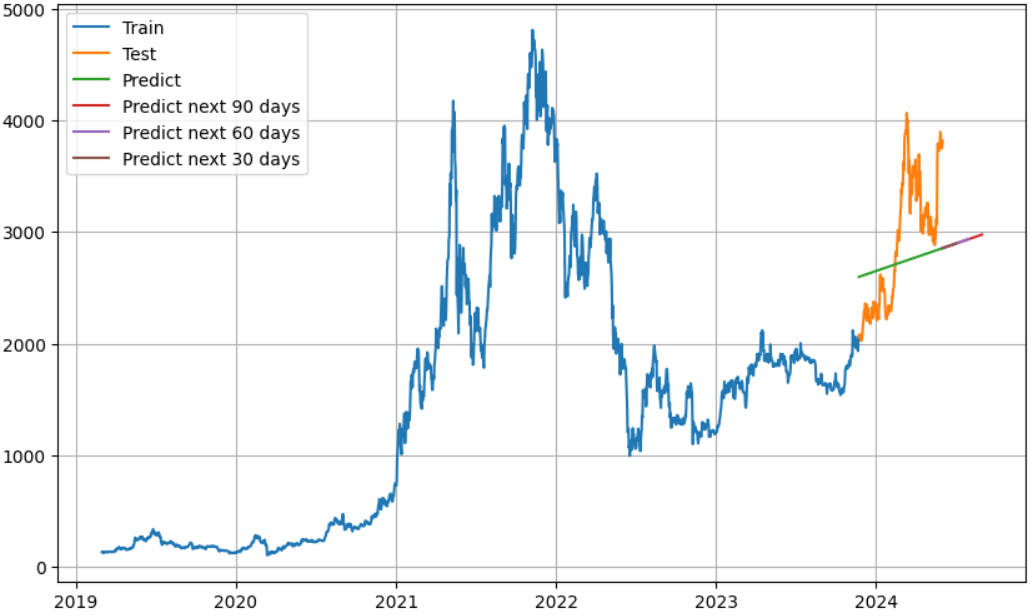
\includegraphics[width=\linewidth]{bibliography/Images/LR_ETH_91.PNG}
		\caption{LR model's result with 9:1 splitting proportion}
	\end{minipage}
\end{figure}
\begin{figure}[H]
	\centering
	\begin{minipage}{0.6\linewidth}
		\centering
		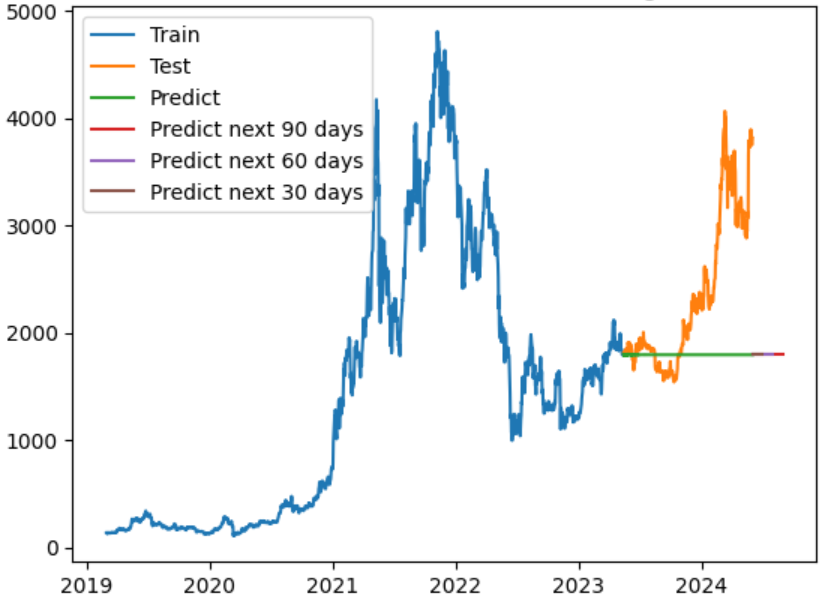
\includegraphics[width=\linewidth]{bibliography/Images/ARIMA_ETH_82.PNG}
		\caption{ARIMA model's result with 8:2 splitting proportion}
	\end{minipage}
\end{figure}
\begin{figure}[H]
	\centering
	\begin{minipage}{0.6\linewidth}
		\centering
		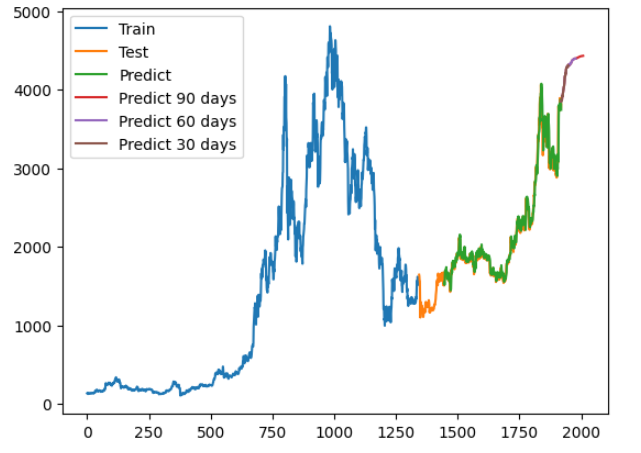
\includegraphics[width=\linewidth]{bibliography/Images/RNN_ETH_73.PNG}
		\caption{RNN model's result with 7:3 splitting proportion}
	\end{minipage}
\end{figure}
\begin{figure}[H]
	\centering
	\begin{minipage}{0.6\linewidth}
		\centering
		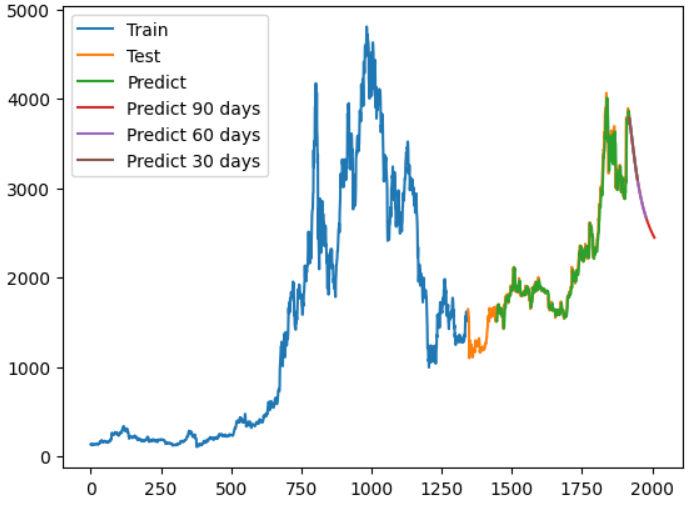
\includegraphics[width=\linewidth]{bibliography/Images/GRU_ETH_73.PNG}
		\caption{GRU model's result with 7:3 splitting proportion}
	\end{minipage}
\end{figure}
\begin{figure}[H]
	\centering
	\begin{minipage}{0.6\linewidth}
		\centering
		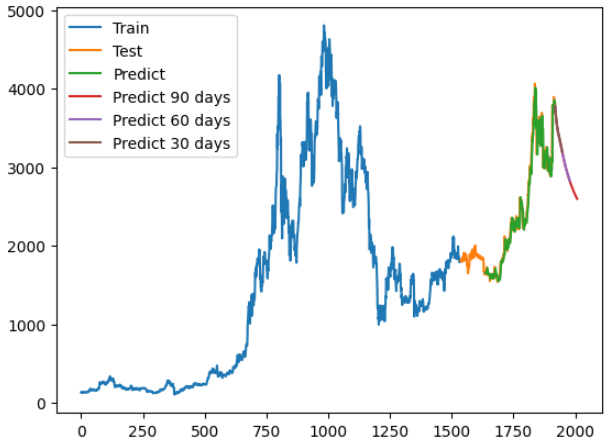
\includegraphics[width=\linewidth]{bibliography/Images/LSTM_ETH_82.PNG}
		\caption{LSTM model's result with 8:2 splitting proportion}
	\end{minipage}
\end{figure}
\begin{figure}[H]
	\centering
	\begin{minipage}{0.6\linewidth}
		\centering
		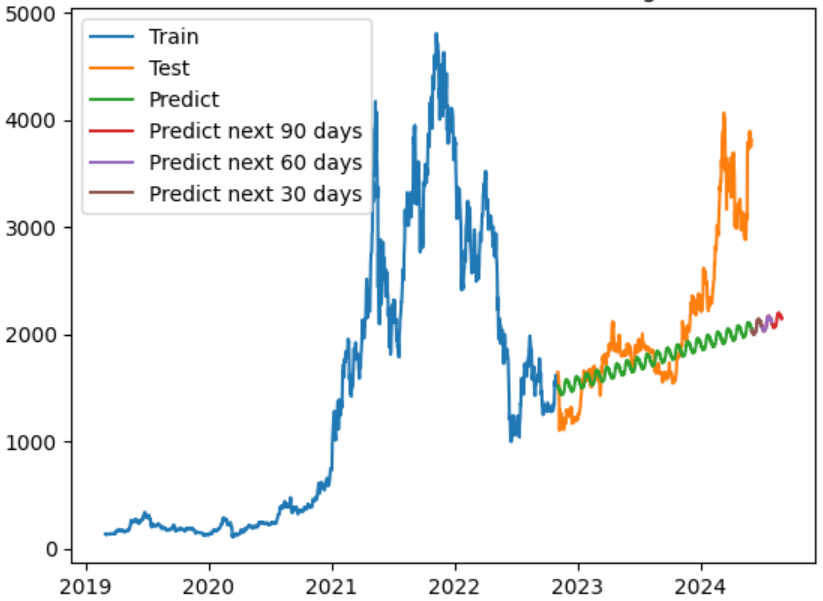
\includegraphics[width=\linewidth]{bibliography/Images/SARIMAX_ETH_73.PNG}
		\caption{SARIMAX model's result with 7:3 splitting proportion}
	\end{minipage}
\end{figure}
\begin{figure}[H]
	\centering
	\begin{minipage}{0.6\linewidth}
		\centering
		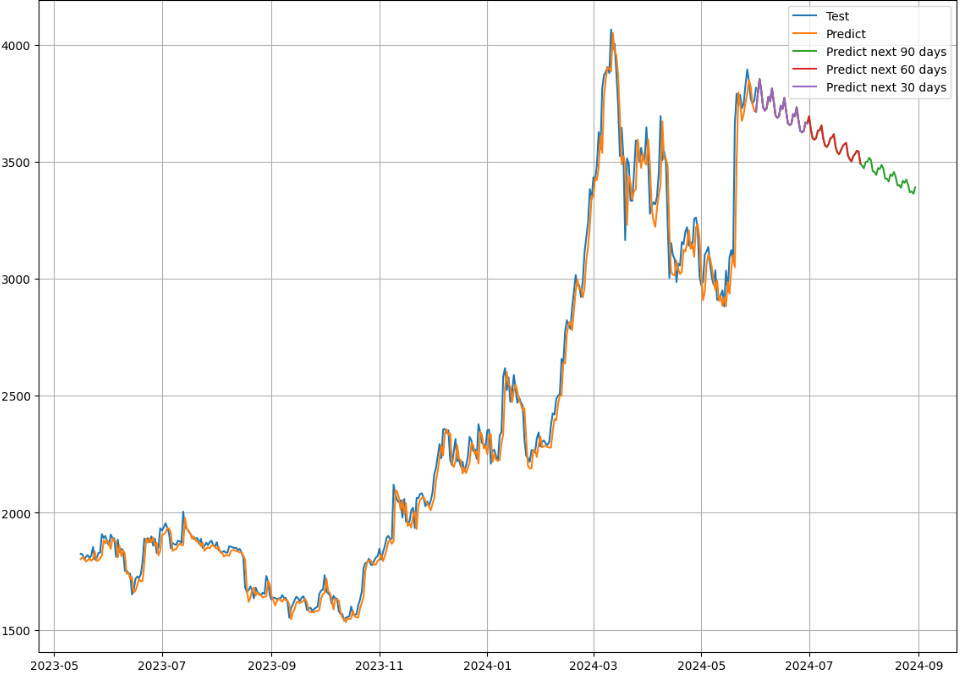
\includegraphics[width=\linewidth]{bibliography/Images/NBEATS_ETH_82.PNG}
		\caption{NBEATS model's result with 8:2 splitting proportion}
	\end{minipage}
\end{figure}
\begin{figure}[H]
	\centering
	\begin{minipage}{0.6\linewidth}
		\centering
		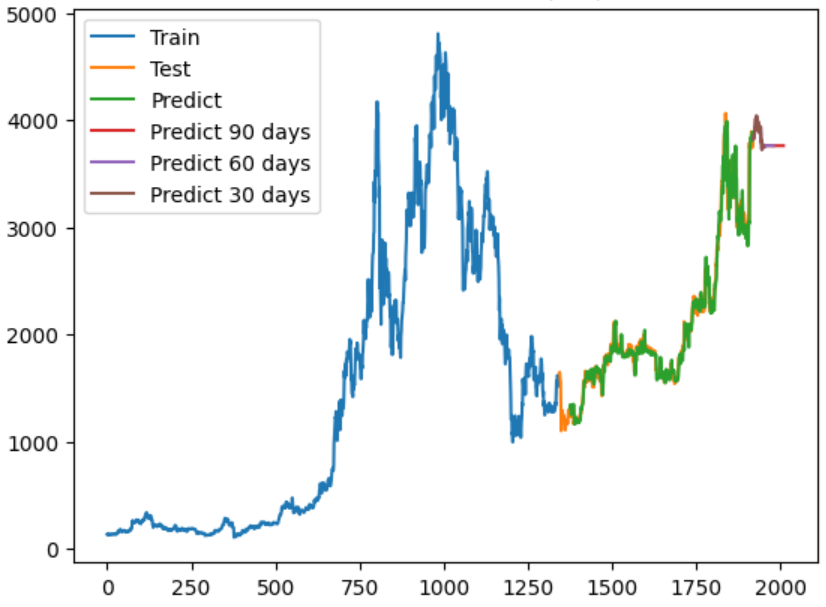
\includegraphics[width=\linewidth]{bibliography/Images/RF_ETH_73.PNG}
		\caption{RF model's result with 7:3 splitting proportion}
	\end{minipage}
\end{figure}
\subsection{BNB/USD Dataset}
\begin{table}[H]
	\centering
	\begin{tabular}{|c|c|c|c|c|}
		\hline
		\multicolumn{5}{|c|}{\textbf{BNB/USD Dataset's Evaluation}}\\
		\hline
		\centering Model & Training:Testing & RMSE & MAPE (\%) & MAE\\
		\hline
		\multirow{2}{*}{LR} & 7:3 & 250.28 &  86.40 &  230.56\\ & 8:2 & 196.35 & 69.72 & 178.19 \\ & \textbf{9:1} & \textbf{131.96} & \textbf{32.73} & \textbf{124.74}\\
		\hline
		\multirow{2}{*}{ARIMA} & \textbf{7:3} & \textbf{116.76} & \textbf{26.33} & \textbf{86.35} \\ & 8:2 & 141.84 & 30.34 & 107.94 \\ & 9:1 & 242.19 & 38.67 & 195.64\\
		\hline
		\multirow{2}{*}{RNN} & 7:3 & 13.03 & 2.86 & 9.26\\ & \textbf{8:2}& \textbf{13.35} & \textbf{2.05} & \textbf{7.91} \\ & 9:1 & 21.46 & 2.54 & 14.21\\
		\hline
		\multirow{2}{*}{GRU} & \textbf{7:3}	& \textbf{11.49} & \textbf{1.87} &  \textbf{6.81} \\ & 8:2 & 13.09 & 2.00 & 7.81 \\ & 9:1 & 20.90  & 2.56 & 14.38\\
		\hline
		\multirow{2}{*}{LSTM} & 7:3 &  12.17 &  2.79 & 8.84 \\ & \textbf{8:2} &  \textbf{13.36} & \textbf{1.97} & \textbf{7.86} \\ & 9:1 &  25.26  & 3.49 & 19.75\\
		\hline
		\multirow{2}{*}{SARIMAX} & \textbf{7:3}	& \textbf{119.44} & \textbf{37.61} &  \textbf{105.42} \\ & 8:2 & 125.43 & 35.96 & 111.44 \\ & 9:1 & 230.67 &  36.82 & 186.24\\
		\hline
		\multirow{2}{*}{NBEATS} & 7:3 & 11.23 & 2.00 & 6.78 \\ & \textbf{8:2} & \textbf{11.90} & \textbf{1.86} & \textbf{6.75} \\ & 9:1 & 15.30	& 2.11 & 9.46 \\
		\hline
		\multirow{2}{*}{RF} & 7:3 & 12.96 & 2.87 & 9.05 \\ & \textbf{8:2} & \textbf{13.45} & \textbf{2.47} & \textbf{8.32} \\ & 9:1 & 17.45 & 2.45 & 11.20 \\
		\hline
	\end{tabular}
	\caption{BNB/USD Dataset's Evaluation}
	\label{ethresult}
\end{table}
\begin{figure}[H]
	\centering
	\begin{minipage}{0.6\linewidth}
		\centering
		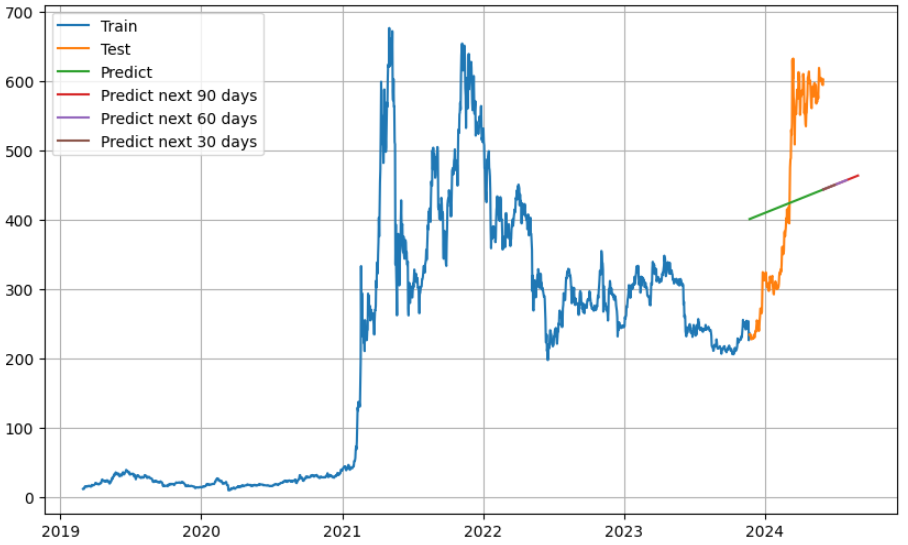
\includegraphics[width=\linewidth]{bibliography/Images/LR_BNB_91.PNG}
		\caption{LR model's result with 9:1 splitting proportion}
	\end{minipage}
\end{figure}
\begin{figure}[H]
	\centering
	\begin{minipage}{0.6\linewidth}
		\centering
		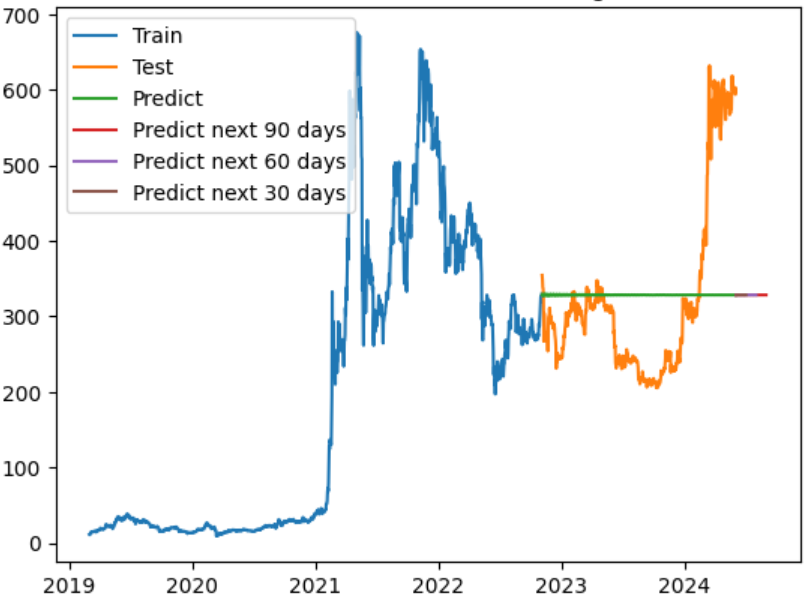
\includegraphics[width=\linewidth]{bibliography/Images/ARIMA_BNB_73.PNG}
		\caption{ARIMA model's result with 7:3 splitting proportion}
	\end{minipage}
\end{figure}
\begin{figure}[H]
	\centering
	\begin{minipage}{0.6\linewidth}
		\centering
		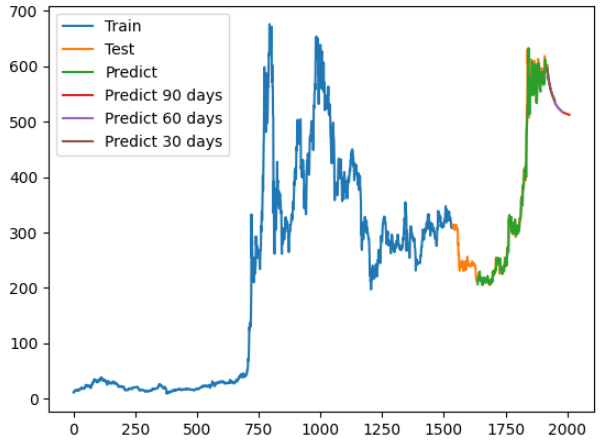
\includegraphics[width=\linewidth]{bibliography/Images/RNN_BNB_82.PNG}
		\caption{RNN model's result with 8:2 splitting proportion}
	\end{minipage}
\end{figure}
\begin{figure}[H]
	\centering
	\begin{minipage}{0.6\linewidth}
		\centering
		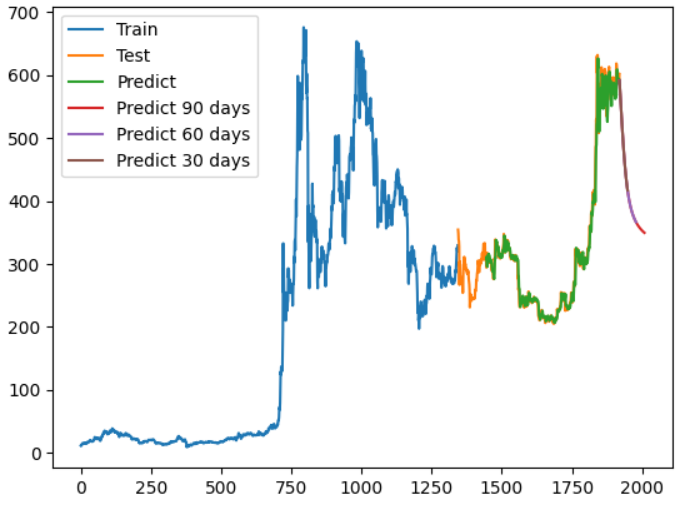
\includegraphics[width=\linewidth]{bibliography/Images/GRU_BNB_73.PNG}
		\caption{GRU model's result with 7:3 splitting proportion}
	\end{minipage}
\end{figure}
\begin{figure}[H]
	\centering
	\begin{minipage}{0.6\linewidth}
		\centering
		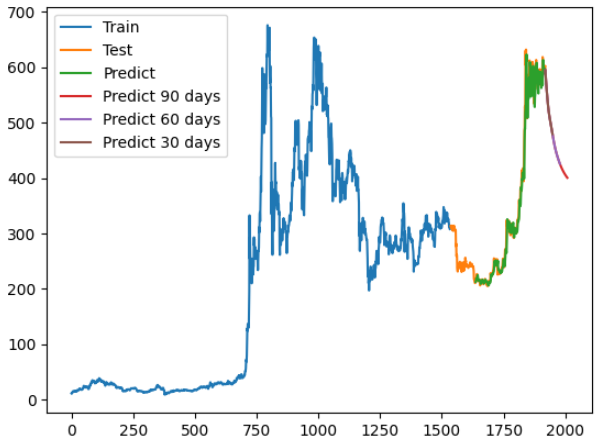
\includegraphics[width=\linewidth]{bibliography/Images/LSTM_BNB_82.PNG}
		\caption{LSTM model's result with 8:2 splitting proportion}
	\end{minipage}
\end{figure}
\begin{figure}[H]
	\centering
	\begin{minipage}{0.6\linewidth}
		\centering
		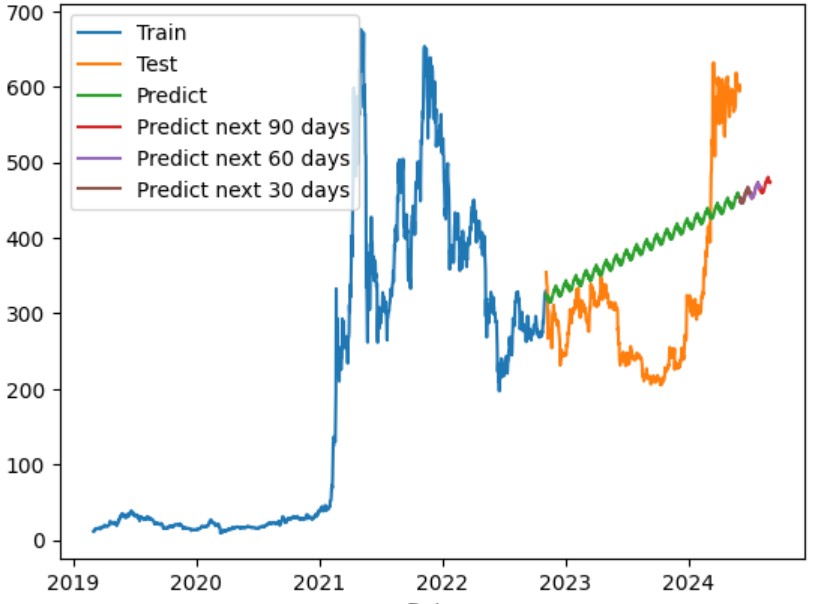
\includegraphics[width=\linewidth]{bibliography/Images/SARIMAX_BNB_73.PNG}
		\caption{SARIMAX model's result with 7:3 splitting proportion}
	\end{minipage}
\end{figure}
\begin{figure}[H]
	\centering
	\begin{minipage}{0.6\linewidth}
		\centering
		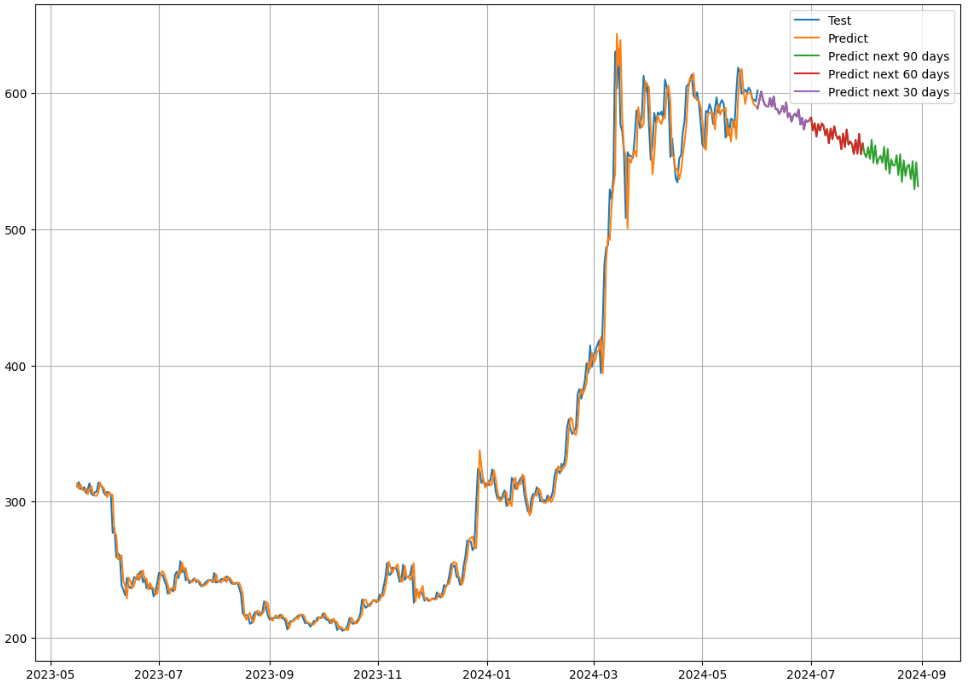
\includegraphics[width=\linewidth]{bibliography/Images/NBEATS_BNB_82.PNG}
		\caption{NBEATS model's result with 8:2 splitting proportion}
	\end{minipage}
\end{figure}
\begin{figure}[H]
	\centering
	\begin{minipage}{0.6\linewidth}
		\centering
		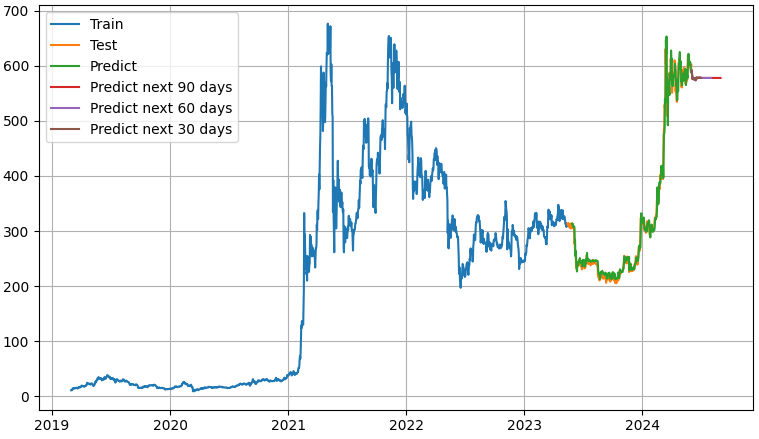
\includegraphics[width=\linewidth]{bibliography/Images/RF_BNB_82.PNG}
		\caption{RF model's result with 8:2 splitting proportion}
	\end{minipage}
\end{figure}

\section{Conclusion}
\subsection{Summary}
In the endeavor to forecast cryptocurrency prices, various methodologies have been explored, ranging from traditional statistical models to advanced machine learning algorithms. Among the models tested, including Linear Regression (LR), Autoregressive Integrated Moving Average (ARIMA), Recurrent Neural Network (RNN), Gated Recurrent Unit (GRU), Long Short-Term Memory (LSTM), Seasonal Autoregressive Integrated Moving Average with eXogenous factors (SARIMAX), Neural Basis Expansion Analysis Time Series (NBEATS), and Random Forest (RF), it is evident that SARIMAX, NBEATS, and RF are the most promising and effective for predicting cryptocurrency prices.\\
The complexities of cryptocurrency price forecasting, driven by the volatility and unpredictability of financial markets, require models that can detect subtle patterns and relationships in the data. SARIMAX excels in managing complex relationships, offering robust predictions. NBEATS, with its capacity to capture sequential dependencies, shows remarkable performance in forecasting cryptocurrency prices. The implementation of ensemble learning through Random Forest (RF) enhances predictive capabilities, providing collective insights that surpass those of individual models.\\
Evaluation metrics, such as RMSE, MAPE, and MAE, reveal that SARIMAX, NBEATS, and RF consistently achieve superior performance in various aspects of forecasting accuracy. Their ability to handle the inherent uncertainties of cryptocurrency markets makes them powerful tools for investors and analysts seeking reliable predictions.
\subsection{Future Considerations}
In our future research, it is essential to focus on further optimizing the models discussed earlier. This optimization should specifically target:\\
\indent\textbullet\ Improving model accuracy. Although the aforementioned algorithms have shown promising results in predicting stock prices, there is a need to enhance the model's accuracy to achieve more precise forecasting outcomes.\\
\indent\textbullet\ Investigating alternative machine learning algorithms or ensemble techniques. Utilizing ensemble techniques, such as combining multiple models or employing various ensemble learning methods, can enhance the robustness and accuracy of the forecasts.\\
\indent\textbullet\ Exploring new forecasting models. The field of forecasting is continually evolving, with new algorithms and models being developed. It is important to stay informed about these advancements and investigate new forecasting models that may offer better accuracy and performance. \\
By continuously exploring and integrating new features, data sources, and modeling techniques, we can aim for ongoing optimization of the forecasting models, thereby improving their ability to predict stock prices with greater precision and reliability.
\section*{Acknowledgment}
\addcontentsline{toc}{section}{Acknowledgment}
We would like to express our sincere gratitude to \textbf{Assoc. Prof. Dr. Nguyen Dinh Thuan} and \textbf{Mr. Nguyen Minh Nhut} for their invaluable guidance, support, and expertise throughout the research process of "Using Forecasting Models in Cryptocurrency Price Prediction." Their insightful feedback and unwavering encouragement have been instrumental in shaping this study. 
\\\textbf{Assoc. Prof. Dr. Nguyen Dinh Thuan}'s profound have provided invaluable insights into the intricacies of cryptocurrency markets and forecasting methodologies. His mentorship has been truly invaluable.
\\We are also deeply thankful to \textbf{Mr. Nguyen Minh Nhut} for his technical assistance, dedication, and relentless pursuit of excellence. His expertise has significantly enhanced the quality and rigor of our research.
\\This research endeavor stands as a testament to the indispensable guidance and contributions of our esteemed mentors. We extend our sincere gratitude to all involved for their invaluable assistance, unwavering encouragement, and steadfast belief in the significance of our research.


\begin{thebibliography}{00}
	
	\bibitem{b1} 
	M. Iqbal, M. S. Iqbal, F. H. Jaskani, K. Iqbal, and A. Hassan, ``Time-Series Prediction of Cryptocurrency Market using Machine Learning Techniques,'' 07 Jul. 2021. [Online]. Available: \url{https://eudl.eu/pdf/10.4108/eai.7-7-2021.170286}
	
	\bibitem{b2} 
	H. N. Gudavalli and K. V. R. Kancherla, ``Predicting Cryptocurrency Prices with Machine Learning Algorithms: A Comparative Analysis,'' Jun. 2023. [Online]. Available: \url{https://www.diva-portal.org/smash/get/diva2:1778251/FULLTEXT03.pdf}
	
	\bibitem{b3} 
	J. Zhu, ``Bitcoin Price Prediction: ARIMA \& SARIMA vs Linear Regression,'' Dec. 2023. [Online]. Available: \url{https://www.researchgate.net/publication/376887838_Bitcoin_Price_Prediction_ARIMA_SARIMA_vs_Linear_Regression}
	
	\bibitem{b4} 
	N. H. Gawali, ``Bitcoin Price Prediction using Neural Network,'' 2021. [Online]. Available: \url{https://norma.ncirl.ie/6125/1/namratagawali.pdf}
	
	\bibitem{b5}
	A. Bulatov, ``Forecasting Bitcoin Prices Using N-BEATS Deep Learning Architecture,'' 12 Dec. 2020. [Online]. Available: \url{https://source.sheridancollege.ca/cgi/viewcontent.cgi?article=1008&context=fast_sw_mobile_computing_theses}
	
	\bibitem{b6}
	J.~R.~Evans, \textit{Business Analytics (1st Edition)}, February 2012.
	
	\bibitem{b7}
	R.~J.~Hyndman and G.~Athanasopoulos, \textit{Forecasting: Principles and Practice (2nd Edition)}, April 2018.
	
	\bibitem{b8}
	F.~R.~Alharbi and D.~Csala, ``A Seasonal Autoregressive Integrated Moving Average with Exogenous Factors (SARIMAX) Forecasting Model-Based Time Series Approach,'' 16 Oct. 2022.
	
	\bibitem{b9}
	Learn AI, ``Random Forest Algorithm,'' 14 Jan. 2023. [Online]. Available: \url{https://medium.com/@divakar1591/random-forest-algorithm-772d3e5568af}
	
	\bibitem{b10}
	A.~Amidi and S.~Amidi, ``Recurrent Neural Networks Cheatsheet,'' [Online]. Available: \url{https://stanford.edu/~shervine/teaching/cs-230/cheatsheet-recurrent-neural-networks?fbclid=IwAR369BvCjGFZ3Ag0x_muwXsbboSIPrHdZd87f_6R4OZGPj_1O7mMFGk3eP0}
	
	\bibitem{b11}
	A.~Saxena, ``Introduction to Long Short-Term Memory (LSTM),'' 18 Jan. 2023. [Online]. Available: \url{https://medium.com/analytics-vidhya/introduction-to-long-short-term-memory-lstm-a8052cd0d4cd}
	
	\bibitem{b12}
	D.~Kharazi, ``Gated Recurrent Units,'' [Online]. Available: \url{https://dkharazi.github.io/notes/ml/nlp/gru?fbclid=IwAR38A4PFm6FAUz_PSeJECQsTdqAhLlqYfXtHyhYefcTwSF52MKHtDnV2e68}
	
	\bibitem{b13}
	A.-R.~Bawa, E.~A.~Sarsah, and A.~Yunus, ``Global Horizontal Irradiance Trend and Its 3 Days Forecast in Northern Ghana Using the 'NeuralForecast' Python Library,'' Nov. 2022. [Online]. Available: \url{https://www.irjmets.com/uploadedfiles/paper//issue_11_november_2022/31348/final/fin_irjmets1669101800.pdf}
	
\end{thebibliography}
\EOD

\end{document}
